\begin{figure}[t]
\begin{centering}
    % \subfloat[this will show up directly below the image]
    {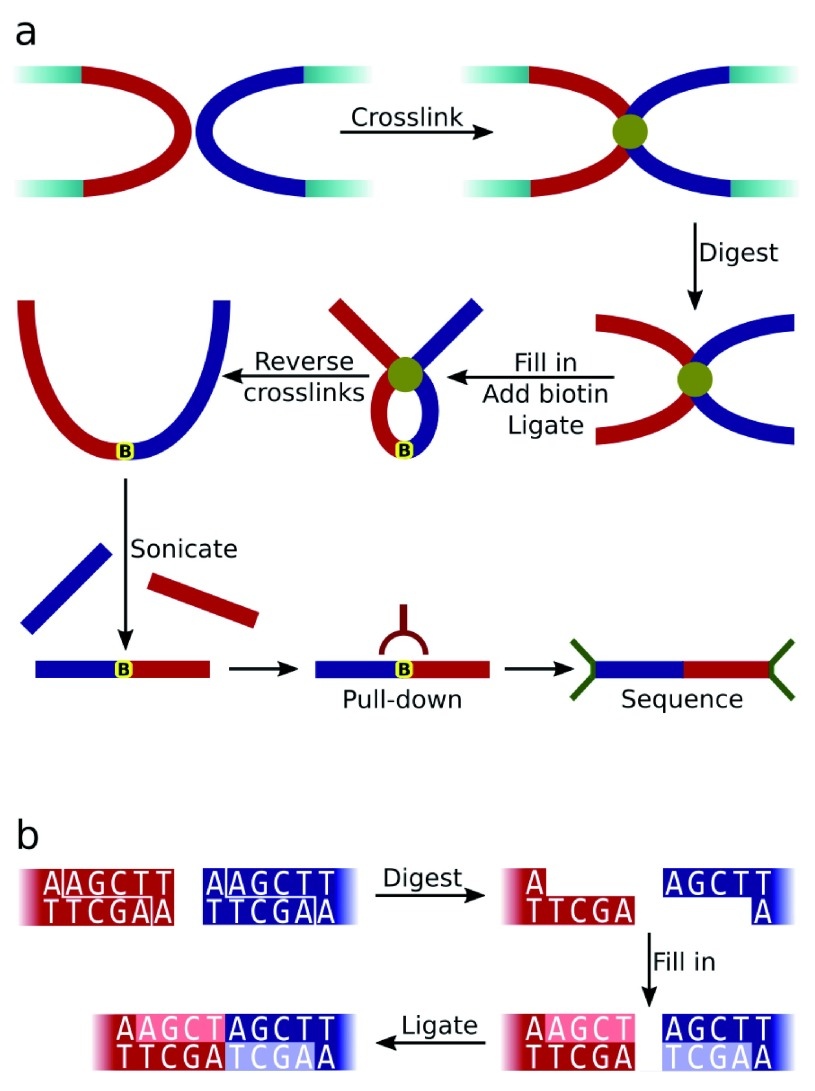
\includegraphics[scale=4]{figures/background/f1000research-4-7903-g0000.jpg}}
    \caption[Summarised Hi-C protocol]
    {\textbf{a)} Diagram summarising the Hi-C experimental protocol. The red
    and blue rectangles represent cross-linked restriction fragments while the
    yellow marker shows the position of biotin incorporation. \\ \\ Image and
    description taken from \cite{wingett2015hicup}.}
    \label{fig:HiC}
    \todo{rewrite the description in my own words}

    \todo{remove the b part from the image}
\end{centering}
\end{figure}

